\documentclass[12pt, twoside]{article}
% \documentclass[12pt, twoside]{article}
\usepackage[letterpaper, margin=1in, headsep=0.2in]{geometry}
\setlength{\headheight}{0.6in}
%\usepackage[english]{babel}
\usepackage[utf8]{inputenc}
\usepackage{microtype}
\usepackage{amsmath}
\usepackage{amssymb}
%\usepackage{amsfonts}
\usepackage[nomessages]{fp} %\FPeval{\var-name}{2*sin(pi/6)}
\usepackage{siunitx} %units in math. eg 20\milli\meter
\usepackage{yhmath} % for arcs, overparenth command
\usepackage{tikz} %graphics
\usetikzlibrary{quotes, angles, arrows, arrows.meta}
\usepackage{graphicx} %consider setting \graphicspath{{images/}}
\usepackage{parskip} %no paragraph indent
\usepackage{enumitem}
\usepackage{multicol}
\usepackage{venndiagram}

\usepackage{fancyhdr}
\pagestyle{fancy}
\fancyhf{}
\renewcommand{\headrulewidth}{0pt} % disable the underline of the header
\raggedbottom
\hfuzz=2mm %suppresses overfull box warnings

\usepackage{hyperref}
\usepackage{float}

\title{Algebra 2}
\author{Chris Huson}
\date{June 2024}

\fancyhead[LE]{\thepage}
\fancyhead[RO]{\thepage \\ Name: \hspace{1.5cm} \,\\}
\fancyhead[LO]{BECA/Huson/Algebra 2: Regents Preparation \\* 3 June 2024}

\begin{document}
\subsubsection*{Prep \#22 Quiz: Graphing}
\begin{enumerate}[itemsep=0.5cm]
\item Graph $f(x)=80(1.2)^x$ on the set of axes below.
\begin{center}
    \begin{tikzpicture}[scale=0.65, xscale=2, yscale=0.05]
        \draw[gray,thin] (0,0) grid [ystep=40](10,400);
        \draw [thick,->] (0,0)--(10.5,0) node [right] {$x$};
        \draw [thick,->] (0,0)--(0,420) node [above] {$y$};
        \foreach \x in {0,1,...,10} 
            \draw (\x cm,10pt) -- (\x cm,-10pt) node[below] {$\x$};
        \foreach \y in {0,40,...,400} 
            \draw (2pt,\y cm) -- (-2pt,\y cm) node[left] {$\y$};
    \end{tikzpicture}
    \end{center}  \vspace{0.5cm}
    \begin{enumerate}
        \item Draw a horizontal line at $y=240$ and approximate the $x$-value where it intersects the curve. \vspace{1cm}
        \item Using the calulator, find the $x$-value where $f(x)=240$ to the \emph{nearest hundredth}.
    \end{enumerate}

\newpage
\item Graph the functions $f(x) = x^2+x-5$ and $g(x) = -x+3$ on the set of axes below. Mark their intersections and label the points as ordered pairs. \vspace{1cm}
\begin{center}
    \begin{tikzpicture}[scale=0.65]
        \draw[gray,very thin] (-10,-10) grid (10,10);
        \draw [thick,<->] (-10.5,0)--(10.5,0) node [right] {$x$};
        \draw [thick,->] (0,-10)--(0,10.5) node [left] {$y$};
    \end{tikzpicture}
    \end{center}
    Check your work:
    \begin{enumerate}[label=$\square$]
        \item The parabola is drawn precisely and is a smooth curve. 
        \item The line is drawn with a ruler and has the correct $y$-intercept.
        \item There are arrows on the ends of the lines if appropriate.
        \item The intersections are marked with points and labeled as ordered pairs. (parentheses)
    \end{enumerate}


\newpage
\subsubsection*{Prep \#22}
\item The probability that Gary and Jane have a child with blue eyes is 0.25, and the probability that they have a child with blond hair is 0.5. The probability that they have a child with both blue eyes and blond hair is 0.125. Make a table to represent the probabilities. \\[0.25cm]
Given this information, the events blue eyes and blond hair are (select all that apply).
\begin{enumerate}
    \item dependent
    \item independent
    \item mutually exclusive
\end{enumerate} \vspace{3cm}


\item Factor and find the zeros of the polynomial equation.
 $$P(x) = x^4-3x^3-x-3$$\vspace{4cm}

\item Solve the system of equations.
\begin{align*}
    x-2y +3z &= 9 \\
    -x+3y -z &= -6 \\
    2x-5y +5z &= 17 \\
\end{align*}

\newpage
\item Given that $f(x)=3|x|-1$ and $g(x)=0.03x^3-x+1$. Use a calculator to solve the equation $f(x)=g(x)$, rounding to the \emph{nearest hundredth}. %June 2017
\vspace{3cm}
\item Convert between radical and rational exponent forms. (assume $x > 0$)
    \begin{multicols}{2}
    \begin{enumerate}
        \item $\displaystyle \frac{4\sqrt[3]{x^6}}{\sqrt{4x^2}} = $
        \item $\displaystyle \frac{(25x)^{\frac{3}{2}}}{y^{-1}} =$
    \end{enumerate}
    \end{multicols} \vspace{2cm}

\item For $x \ne 0$, which expressions are equivalent to one divided by the sixth root of $x$?
$$\displaystyle I. \frac{\sqrt[6]{x}}{\sqrt[3]{x}} 
\hspace{0.5cm} II. \frac{x^{\frac{1}{6}}}{x^{\frac{1}{3}}} 
\hspace{0.5cm} III. x^{-\frac{1}{6}}$$. \vspace{3cm}

\item Simplify each complex expression to the form $a+bi$.
    \begin{multicols}{2}
    \begin{enumerate}[itemsep=2cm]
        \item $i^3=$
        \item $(1+5i)(2-4i)=$
        \item $(1+3i)^2=$
        \item $6xi^3(-4xi+5)$ %June 2017
    \end{enumerate}
    \end{multicols} \vspace{3cm}


\end{enumerate}
\end{document}